% Copyright (c)  2005-2010 EDF-EADS-PHIMECA.
% Permission is granted to copy, distribute and/or modify this document
% under the terms of the GNU Free Documentation License, Version 1.2
% or any later version published by the Free Software Foundation;
% with no Invariant Sections, no Front-Cover Texts, and no Back-Cover
% Texts.  A copy of the license is included in the section entitled "GNU
% Free Documentation License".
\renewcommand{\etapemethodo}{B}
\renewcommand{\nomfichier}{docref_B221_Graph}
\renewcommand{\titrefiche}{Graphical goodness-of-fit tests : QQ-plot, Kendall Plot and Henry line}

\Header

\MathematicalDescription{

  \underline{\textbf{Goal}} \vspace{2mm}

  This method is concerned with the modelling of a probability distribution of a random vector $\vect{X} = \left( X^1,\ldots,X^{n_X} \right)$. It seeks to verify the compatibility between a sample of data $\left\{ \vect{x}_1,\vect{x}_2,\ldots,\vect{x}_N \right\}$ and a candidate probability distribution previous chosen. Open TURNS enables the use of graphical tools to answer this question in the one dimensional case $n_X =1$, and with a continuous distribution.
  \vspace{2mm}

  \underline{\textbf{Principle}} \vspace{2mm}

  The QQ-plot, and henry line tests are defined in the case to $n_X = 1$. Thus we denote $\vect{X} = X^1 = X$. The first graphical tool provided by Open  TURNS is a QQ-plot (where "QQ" stands for "quantile-quantile"). In the specific case of a Normal distribution (see \otref{docref_B121_DistributionSelection}{standard parametric models}), Henry's line may also be used.

  \textbf{QQ-plot}

  A QQ-Plot is based on the notion of quantile. The $\alpha$-quantile $q_{X}(\alpha)$ of $X$, where $\alpha \in (0, 1)$, is defined as follows:
  $$
  \Prob{ X \leq q_{X}(\alpha)} = \alpha
  $$
  If a sample $\left\{x_1,\ldots,x_N \right\}$ of $X$ is available, the quantile can be estimated empirically:
  \begin{enumerate}
  \item the sample $\left\{x_1,\ldots,x_N \right\}$ is first placed in ascending order, which gives the sample $\left\{ x_{(1)},\ldots,x_{(N)} \right\}$;
  \item then, an estimate of the $\alpha$-quantile is:
    $$
    \widehat{q}_{X}(\alpha) = x_{([N\alpha]+1)}
    $$
    where $[N\alpha]$ denotes the integral part of $N\alpha$.
  \end{enumerate}

  Thus, the $j^\textrm{th}$ smallest value of the sample $x_{(j)}$ is an estimate $\widehat{q}_{X}(\alpha)$ of the $\alpha$-quantile where $\alpha = (j-1)/N$ ($1 < j \leq N$).

  Let us then consider the candidate probability distribution being tested, and let us denote by $F$ its cumulative distribution function. An estimate of the $\alpha$-quantile can be also computed from $F$:
  $$
  \widehat{q}'_{X}(\alpha) = F^{-1} \left( (j-1)/N \right)
  $$
  If $F$ is really the cumulative distribution function of $F$, then $\widehat{q}_{X}(\alpha)$ and $\widehat{q}'_{X}(\alpha)$ should be close. Thus, graphically, the points $\left\{ \left( \widehat{q}_{X}(\alpha),\widehat{q}'_{X}(\alpha)\right),\  \alpha = (j-1)/N,\ 1 < j \leq N \right\}$ should be close to the diagonal.

  The following figure illustrates the principle of a QQ-plot with a sample of size $N=50$. Note that the unit of the two axis is that of the variable $X$ studied; the quantiles determined via $F$ are called here "value of $T$". In this example, the points remain close to the diagonal and the hypothesis "$F$ is the cumulative distribution function of $X$" does not seem irrelevant, even if a more quantitative analysis (see for instance \otref{docref_B222_TestKS}{Kolmogorov-Smirnov goodness-of-fit test}) should be carried out to confirm this.

  \begin{center}
    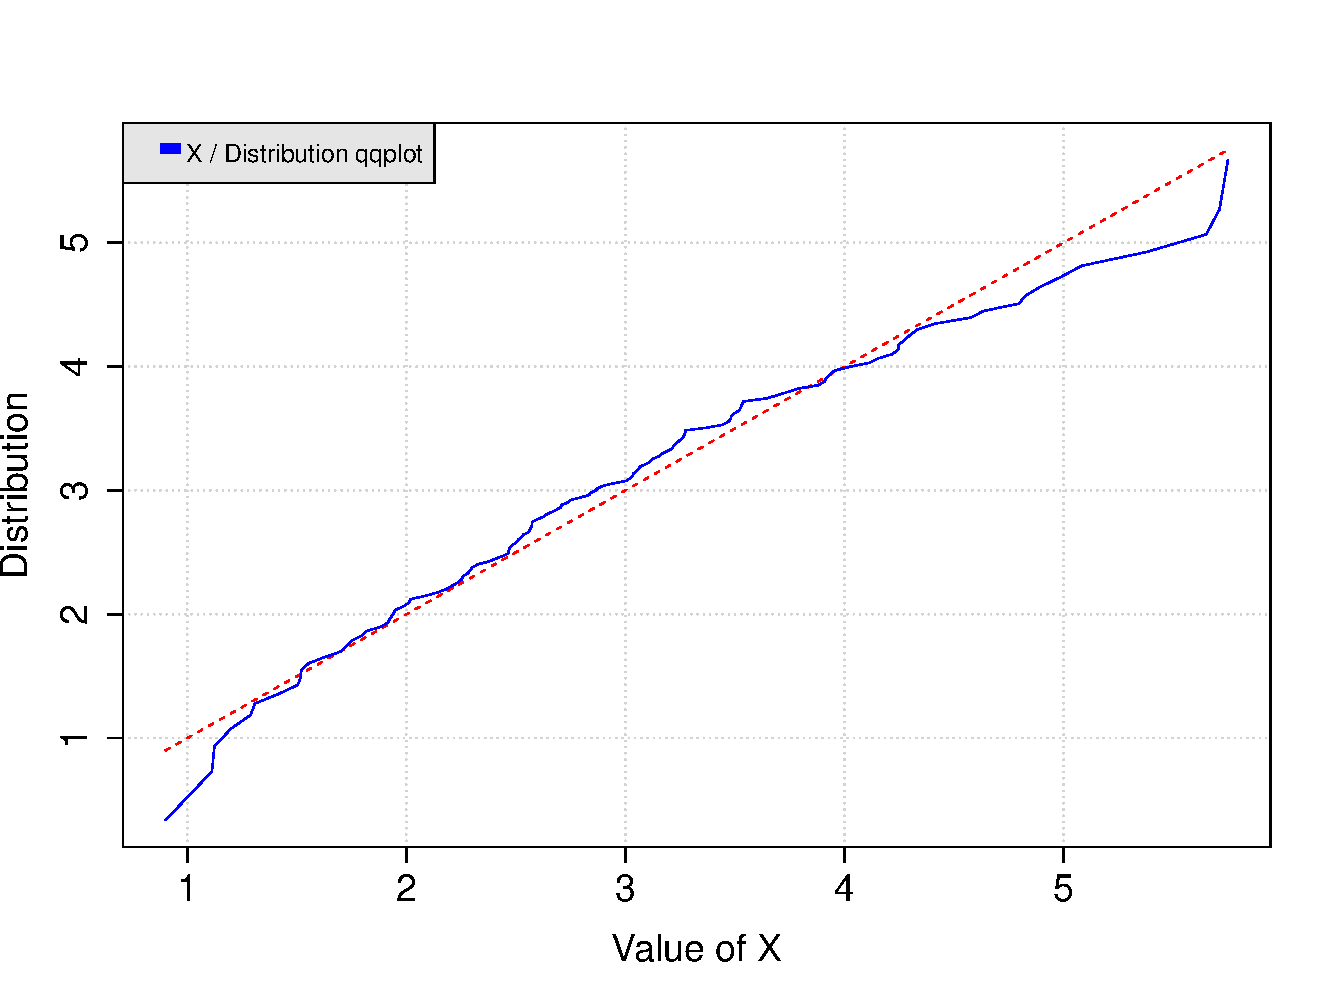
\includegraphics[scale=0.5]{QQplotDistribOk.pdf}
  \end{center}

  In this second example, the candidate distribution function is clearly irrelevant.

  \begin{center}
    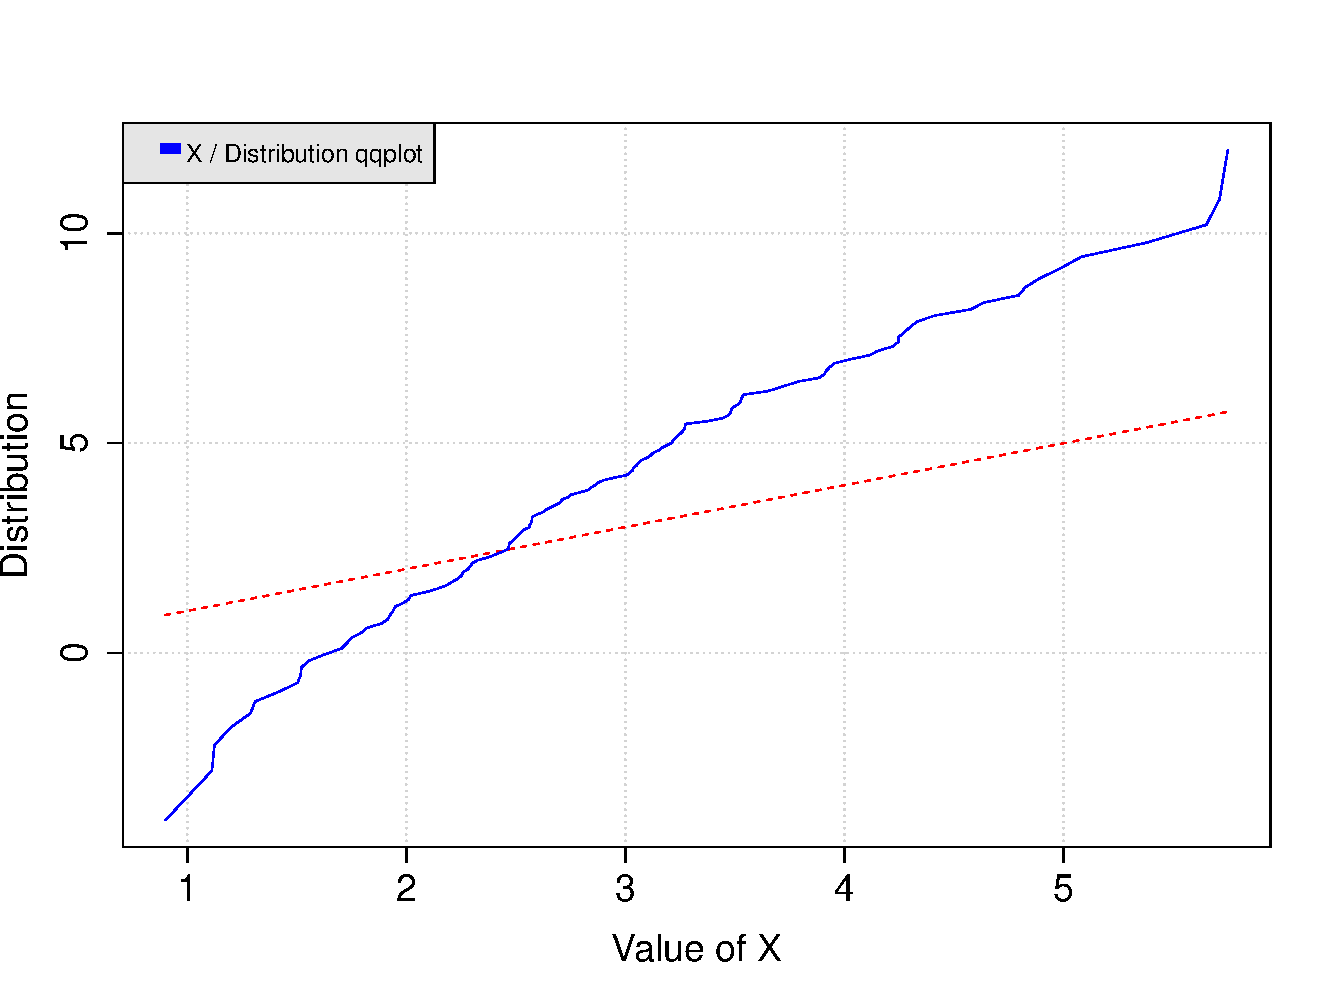
\includegraphics[scale=0.6]{QQplotDistribBad.pdf}
  \end{center}


  \textbf{Henry's line}

  This second graphical tool is only relevant if the candidate distribution function being tested is gaussian. It also uses the ordered sample $\left\{ x_{(1)},\ldots,x_{(N)} \right\}$ introduced for the QQ-plot, and the empirical cumulative distribution function $\widehat{F}_N$ presented in \otref{docref_B11_EmpiricalCDF}{empirical cumulative distribution function}.

  By definition,
  $$
  x_{(j)} = \widehat{F}_N^{-1} \left( \frac{j}{N} \right)
  $$
  Then, let us denote by $\Phi$ the cumulative distribution function of a Normal distribution with mean 0 and standard deviation 1. The quantity $t_{(j)}$ is defined as follows:
  $$
  t_{(j)} = \Phi^{-1} \left( \frac{j}{N} \right)
  $$

  If $X$ is distributed according to a normal probability distribution with mean $\mu$ and standard-deviation $\sigma$, then the points $\left\{ \left( x_{(j)},t_{(j)} \right),\ 1 \leq j \leq N \right\}$ should be close to the line defined by $t = (x-\mu) / \sigma$. This comes from a property of a normal distribution: it the distribution of $X$ is really $\mathcal{N}(\mu,\sigma)$, then the distribution of $(X-\mu) / \sigma$ is $\mathcal{N}(0,1)$.

  The following figure illustrates the principle of Henry's graphical test with a sample of size $N=50$. Note that only the unit of the horizontal axis is that of the variable $X$ studied. In this example, the points remain close to a line and the hypothesis "the distribution function of $X$ is a gaussian one" does not seem irrelevant, even if a more quantitative analysis (see for instance \otref{docref_B222_TestKS}{Kolmogorov-Smirnov goodness-of-fit test}) should be carried out to confirm this.

  \begin{center}
    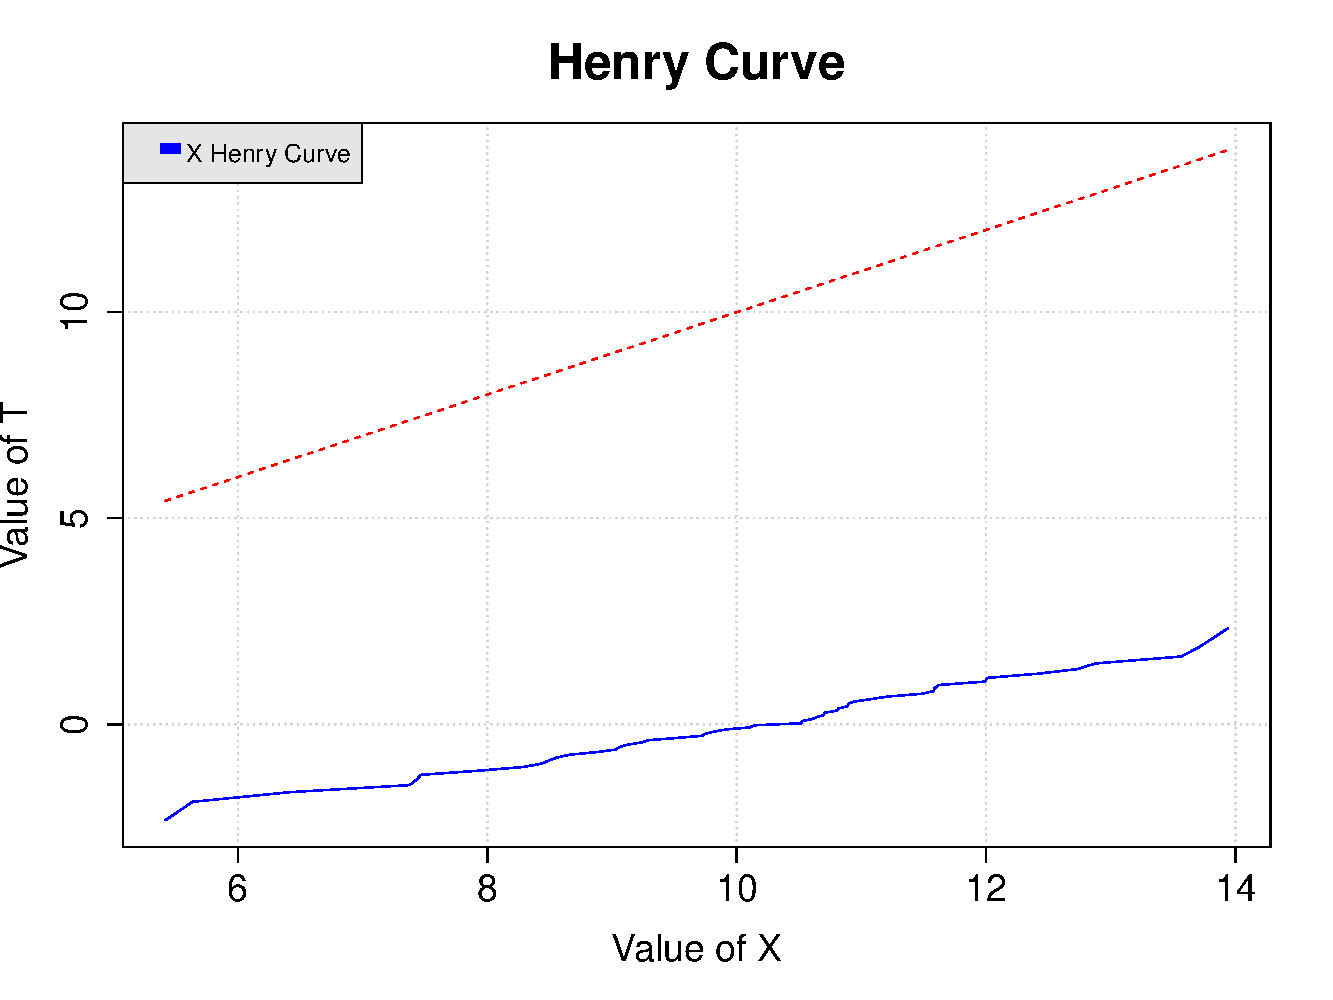
\includegraphics[scale=0.6]{henryGraph.pdf}
  \end{center}

  In this second example, the hypothesis of a gaussian distribution seems far less relevant because of the behaviour for small values of $X$.

  \begin{center}
    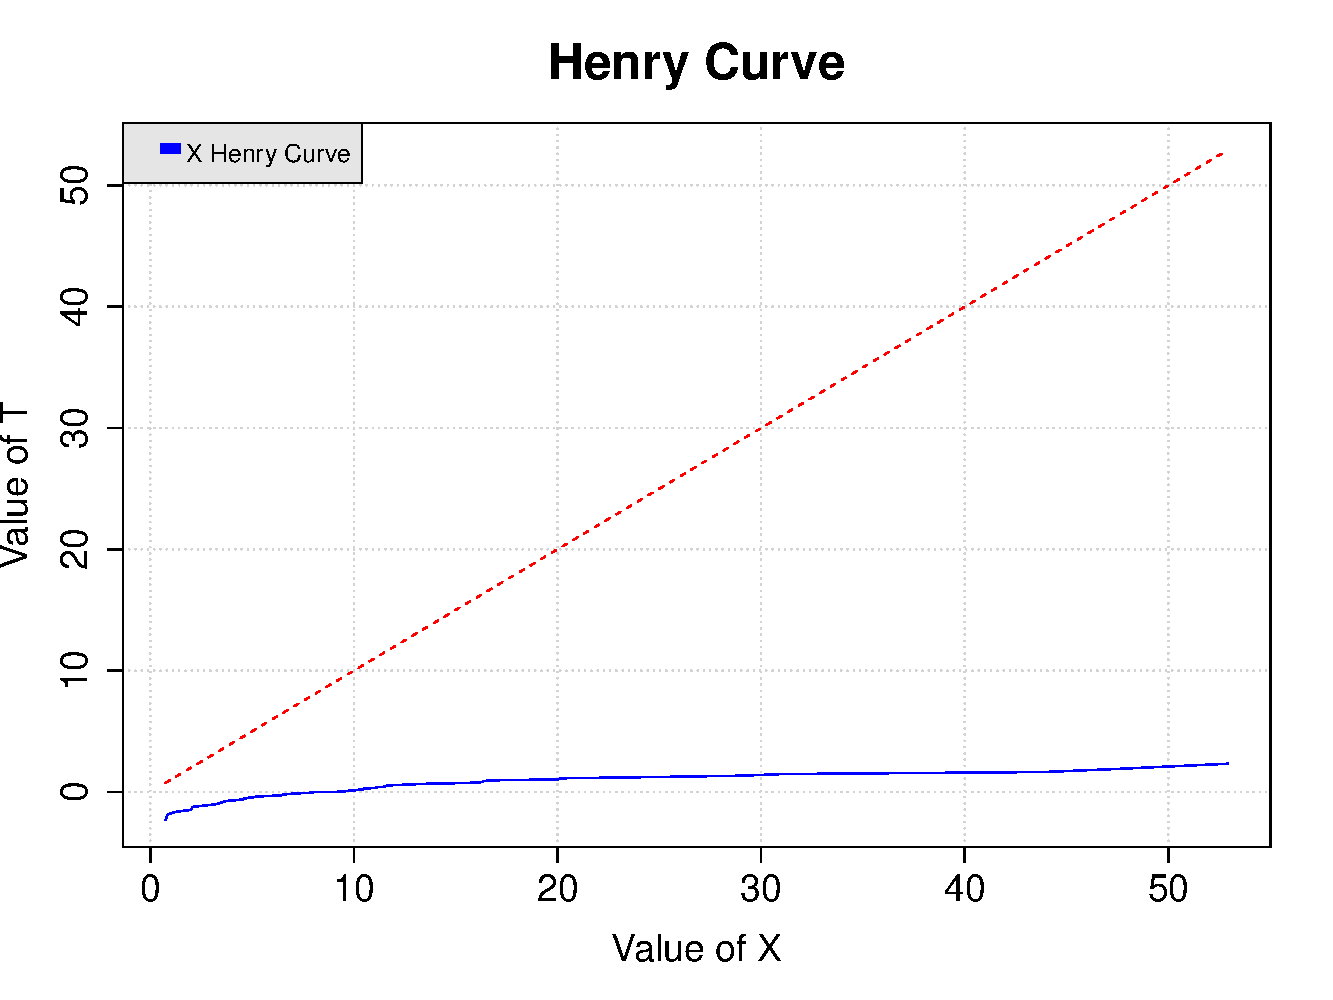
\includegraphics[scale=0.6]{henryBadGraph.pdf}
  \end{center}

  \textbf{Kendall plot}\\

In the bivariate case, the Kendall Ploot test enables to validate the choice of a specific copula model or to verify that two samples share the same copula model.\\
Let $\vect{X}$ be a bivariate random vector which copula is noted $C$.\\

Let $(\vect{X}^i)_{1 \leq i \leq N}$ be a  sample of $\vect{X}$.\\

We note :
$$
\forall i \geq 1, \displaystyle H_i = \frac{1}{n-1} Card \left\{  j \in [1,N], j  \neq i, \, | \, x^j_1 \leq x^i_1 \mbox{ and } x^j_2 \leq x^i_2  \right \}
$$
and $(H_{(1)}, \dots, H_{(N)})$ the  ordered statistics of $(H_1, \dots, H_N)$.\\

The statistic $W_i$ is defined by : 
\begin{equation} \label{Wi}
W_i = N C_{N-1}^{i-1} \int_0^1 t K_0(t)^{i-1} (1-K_0(t))^{n-i} \, dK_0(t)
\end {equation}
where $K_0(t)$ is the cumulative density function of $H_i$. We can show that this is the cumulative density function of the random variate $C(U,V)$ when $U$ and $V$ are independent and follow $Uniform(0,1)$ distributions. \\


In Open TURNS 0.15.0, Eq. (\ref{Wi}) is evaluated with the Monte Carlo sampling method : Open TURNS generates $n$ samples of size $N$ from the bivariate copula $C$, in order to have $n$ realisations of the statistics $H_{(i)},\forall 1 \leq i \leq N$ and have an estimation of $W_i = E[H_{(i)}], \forall i \leq N$. \\

When testing a specific copula with respect to a sample, the Kendall Plot test draws the points $(W_i, H_{(i)})_{1 \leq i \leq N}$. If the points are one the first diagonal, the copula model is validated. \\

When testing whether two samples have the same copula, the Kendall Plot test draws the points $(H^1_{(i)}, H^2_{(i)})_{1 \leq i \leq N}$ respectively associated to the first and second sample. Note that the two samples must have the same size.\\

In Figures  \ref{GoodCop} to \ref{DifCop}, the data 1 and data 2  have been generated from a $Frank(1.5)$ copula, and data 3 from a $Gumbel(4.5)$ copula.\\

Figures \ref{GoodCop} and \ref{BadCop} respectively validates and invalidates the $Frank$ copula model to data 1 and data 2.\\

Figures \ref{SameCop} and \ref{DifCop} respectively validates that data 1 and data 2 share the same copula, and shows that data 1 and data 3 don't share the same copula.

\begin{figure}[H]
  \begin{minipage}{8cm}
    \begin{center}
      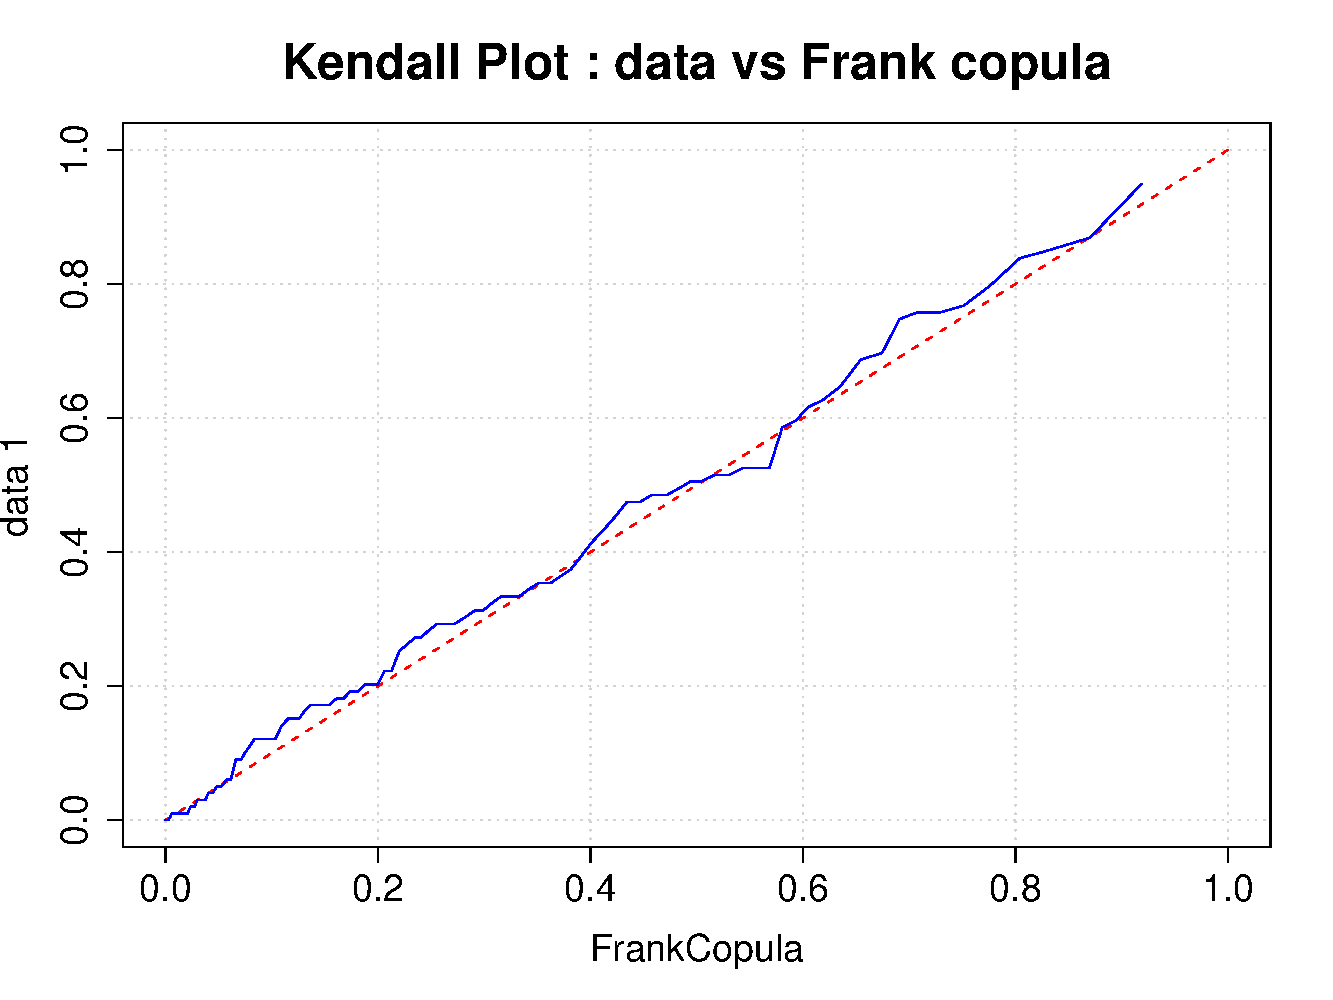
\includegraphics[width=8cm]{KendallPlotCopula.pdf}
    \end{center}
    \caption{The Kendall Plot test validates the use of the Frank copula model for the data 1.}
    \label{GoodCop}
  \end{minipage}
  \hfill
  \begin{minipage}{8cm}
    \begin{center}
      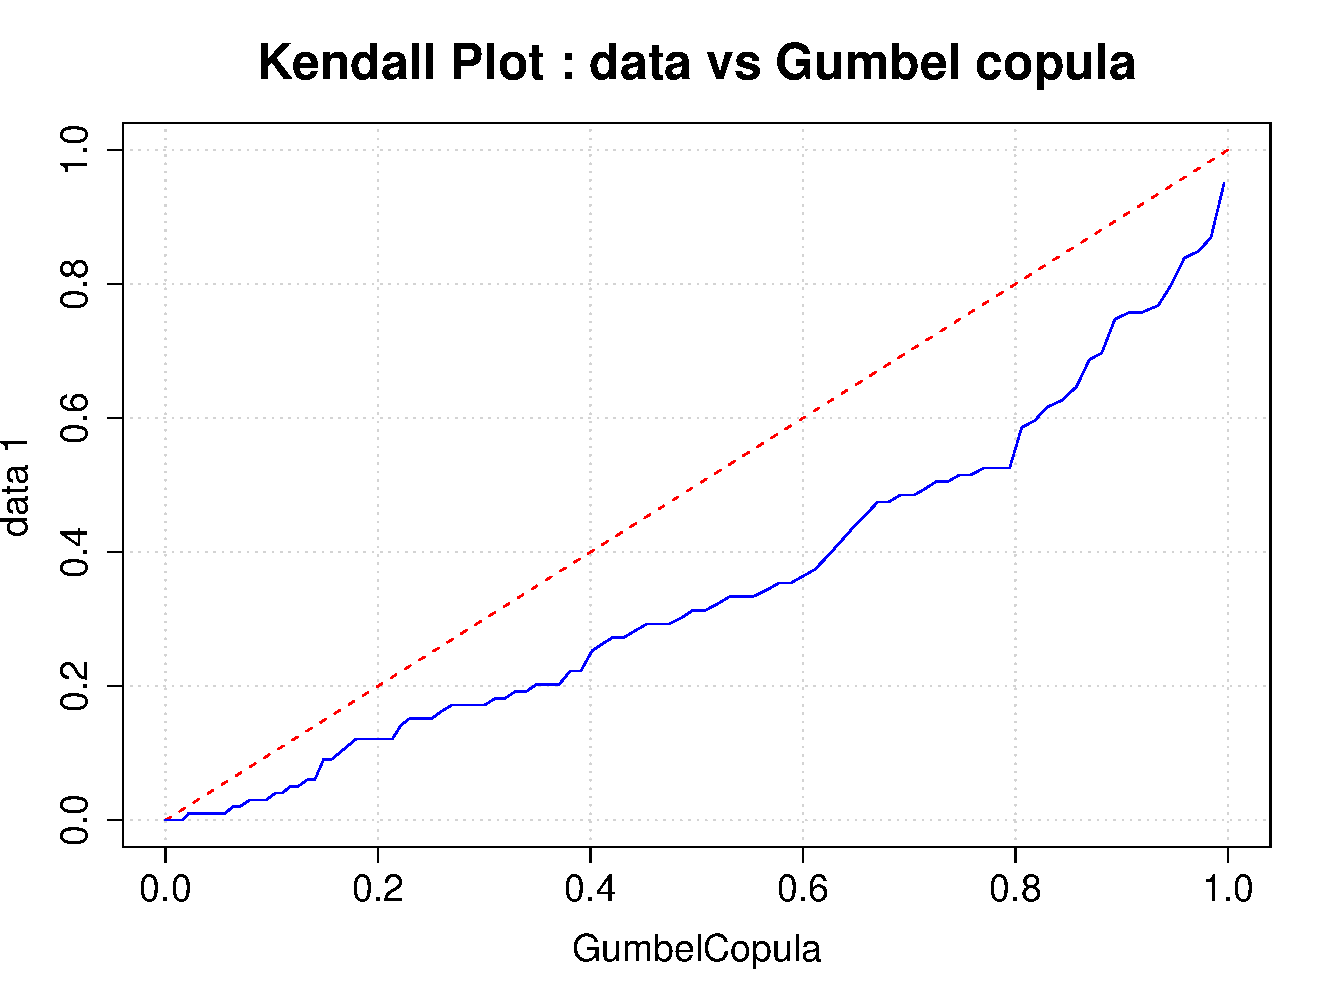
\includegraphics[width=8cm]{KendallPlotCopulaBad.pdf}
    \end{center}
    \caption{The Kendall Plot test invalidates the use of the Frank copula model for the data 1.}
    \label{BadCop}
  \end{minipage}
\end{figure}


\begin{figure}[H]
  \begin{minipage}{8cm}
    \begin{center}
      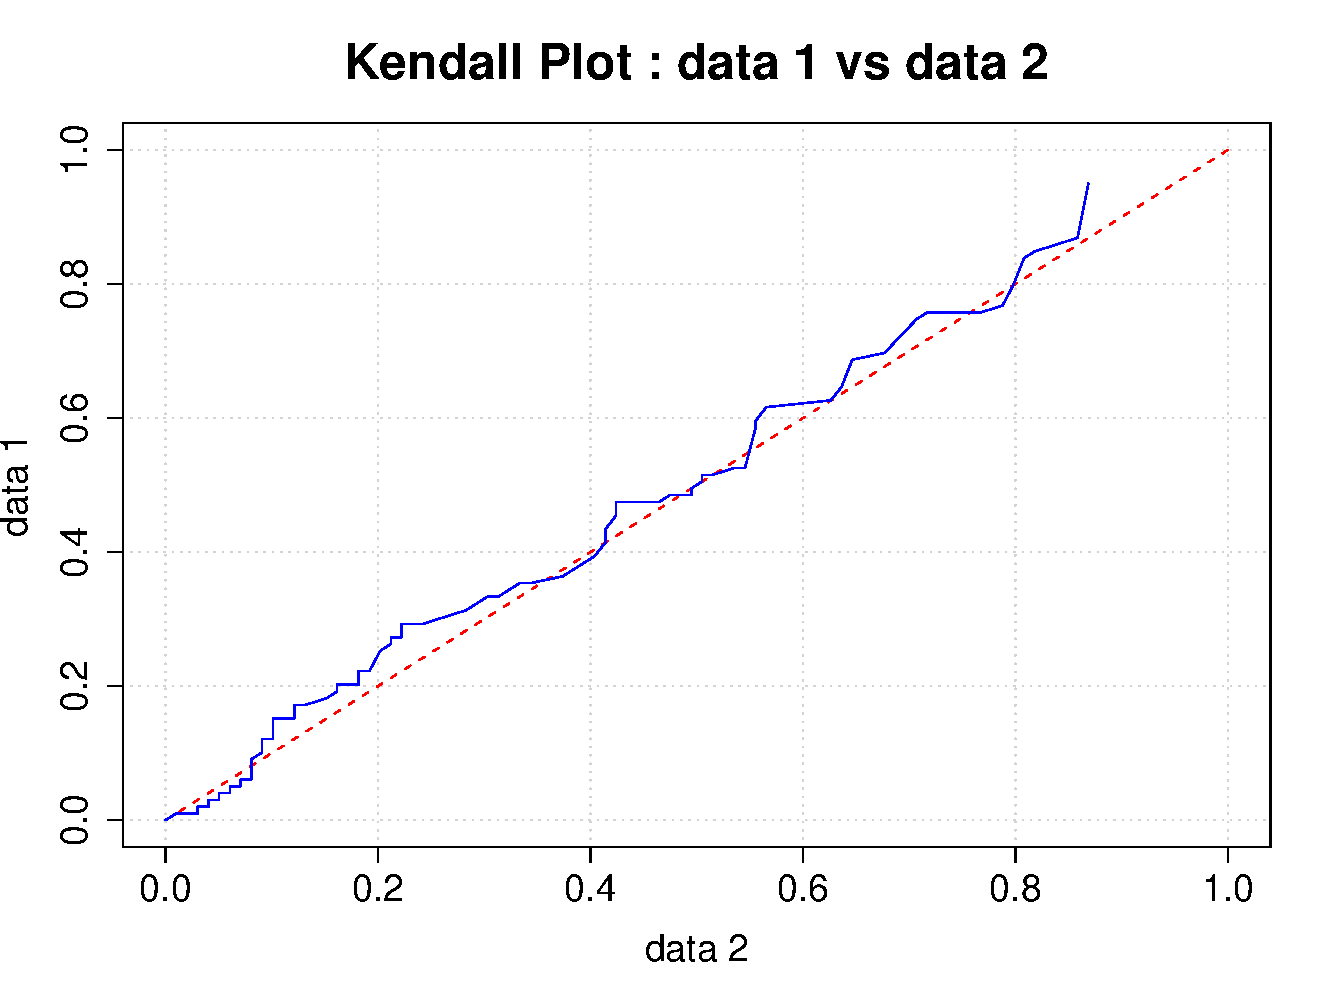
\includegraphics[width=8cm]{KendallPlotSample.pdf}
    \end{center}
    \caption{The Kendall Plot test validates that data 1 and data 2 have the same copula model}.
    \label{SameCop}
  \end{minipage}
  \hfill
  \begin{minipage}{8cm}
    \begin{center}
      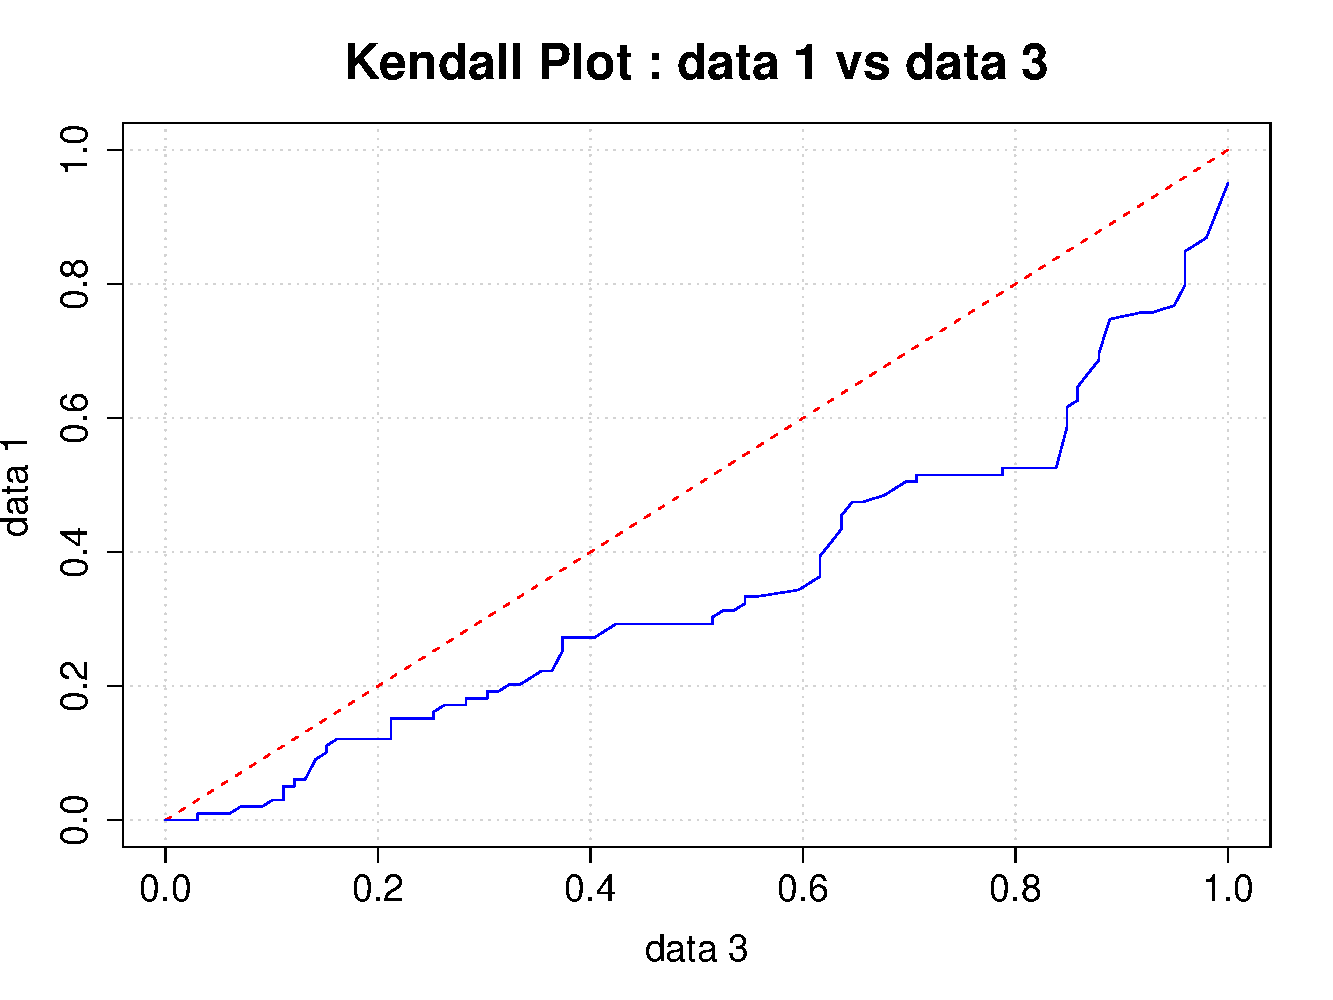
\includegraphics[width=8cm]{KendallPlotSampleBad.pdf}
    \end{center}
    \caption{The Kendall Plot test invalidates that data 1 and data 3 have the same copula model}.
    \label{DifCop}
  \end{minipage}
\end{figure}




Remark :  In the case where you want to test a sample with respect to a specific copula, if the size of the sample is superior to 500, we recommend to use the second form of the Kendall plot test : generate a sample of the proper size from your copula and then test both samples. This way of doing is more efficient.


}
{
-
}

\Methodology{
  This method is used in step B "Quantifying Sources of Uncertainty", to verify if the probability distribution is appropriate to describe the uncertainty of a component $X^i$ of the vector of unknown variables defined in step A "Specifying Criteria and the Case Study". The Kendall Plot is used to validate a copula model.
}
{
  Since QQ-plot and Henry's line are graphical analysis, their conclusion remain obviously subjective. The reader is referred to \otref{docref_B222_TestKS}{Komogorov-Smirnov test}, \otref{docref_B222_TestCVM}{Cramer-Von-Mises test}, \otref{docref_B222_TestAD}{Anderson-Darling test} for a more quantitative analysis.

  The following bibliographical references provide main starting points for further study of this method:
  \begin{itemize}
  \item Saporta G. (1990). "Probabilit�s, Analyse de donn�es et Statistique", Technip
  \item Dixon W.J. \& Massey F.J. (1983) "Introduction to statistical analysis (4th ed.)", McGraw-Hill
  \end{itemize}
}
